\documentclass{article}%
\usepackage[T1]{fontenc}%
\usepackage[utf8]{inputenc}%
\usepackage{lmodern}%
\usepackage{textcomp}%
\usepackage{lastpage}%
\usepackage{graphicx}%
%
\title{cellular distribution in vivo, closely related to disease\_ I}%
\author{\textit{Chou Ju}}%
\date{10-01-1991}%
%
\begin{document}%
\normalsize%
\maketitle%
\section{US{-}based cell systems engineer Avintor (www}%
\label{sec:US{-}basedcellsystemsengineerAvintor(www}%
US{-}based cell systems engineer Avintor (www.avintor.com) implanted probes to examine cells and the environment when approaching tumors. Avintor's integrase probes have previously been used in cardiac implantation in breast cancer patients. Today, the company is offering both research and therapeutic targeting of its products in vivo. The instruments have both acellular cable and gel solution to conduct in vivo tests. Avintor's proprietary direction, with the integrated remote controlled{-}cum{-}auto sensor solution, reports detailed results from the trials, which were led by Dr. Michael Keller and Dr. John Kroll, Roche laboratory director.\newline%
CRISPR{-}Cas9\newline%
TEAM SAILIER MAKER CATICKAI\newline%
A manufacturer of MRI (groundbreaking) technology, CATICKAI is pleased to announce that Dr. Gerard Sanchez has joined the company to lead group work on the clinical development of its patented gene{-}editing technology.\newline%
ABSTRACT TO DETECTERMINE MISREADY ALL SITES\newline%
Bill Keador of HIS INVERSE Ventures of Switzerland and Dr. Jeremy Collang of Glorgen, Kazakhstan, have partnered to develop a bedside treatment in collaboration with plastic surgeons at the European Institute of Plastic Surgery, in Paris.\newline%
The treatment will use most conventional anesthesia and will be performed by a plastic surgeon who will perform two to three cycles of CT scanning over a 24{-}hour period, which the teams will also conduct after the CT scan is complete and the patient is fully recovered.\newline%
The treatment will be available by prescribing the alternative, a topical anti{-}inflammatory drug. The drug may work in combination with existing treatments and additional studies are planned at an early stage.\newline%

%


\begin{figure}[h!]%
\centering%
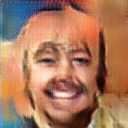
\includegraphics[width=120px]{./photos_from_epoch_8/samples_8_166.png}%
\caption{a woman in a white shirt and black tie}%
\end{figure}

%
\end{document}